\chapter{Setting up and maintaining \ReplicaNextLong{}}\label{ch:replica-next-setup}

This section applies to the \ReplicaNextLong{} dashboard shown in \autoref{fig:next-hardware}.

\begin{figure}[htbp]
    \centering
    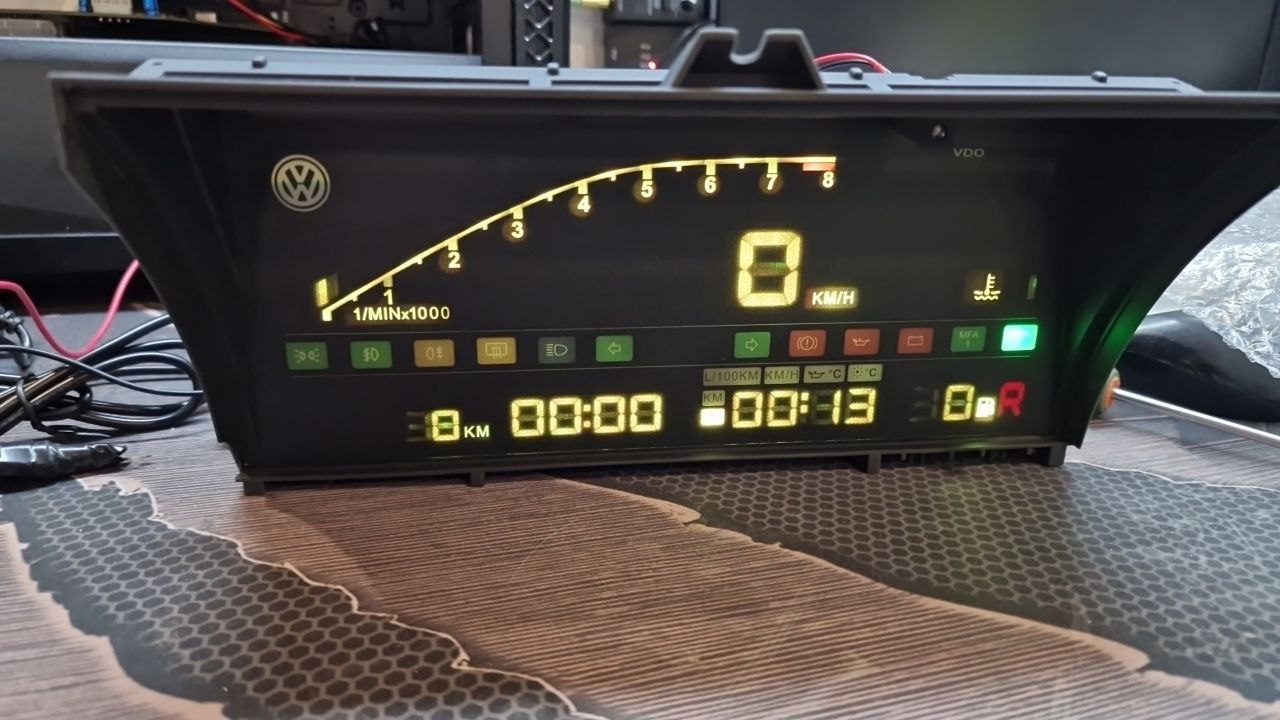
\includegraphics[width=0.6\textwidth]{digifiz_manual/image019.png}
    \caption{\ReplicaNextLong{} dashboard assembly.}
    \label{fig:next-hardware}
\end{figure}

\section{Panel handling}
\begin{itemize}
    \item The UV-printed polycarbonate faceplate must be protected from scratches and foreign objects. Significant damage requires replacement parts from PHOL-LABS Kft and is not treated as a warranty case.
    \item The real-time clock is configured via the Wi-Fi control panel. It resets whenever the permanent supply is disconnected.
\end{itemize}

\section{Wi-Fi control portal}
Configuration, data collection, and firmware management are performed through the embedded web application.
\begin{itemize}
    \item Connect to the dashboard's Wi-Fi access point. Disable mobile data and join \texttt{Digifiz\_AP} (password \texttt{87654321}); some revisions advertise \texttt{PHOL-LABS2} with the same password.
    \item The default IP address is \texttt{192.168.4.1}. If the dashboard is configured to join another network, scan the subnet for an address ending in \texttt{.32} using an IP tools application.
    \item The portal contains three tabs: \emph{WiFi}, \emph{Control}, and \emph{About} (\autoref{fig:next-control-tabs}). The Wi-Fi tab configures network settings and handles firmware uploads; the Control tab adjusts dashboard parameters; the About tab lists author information.
\end{itemize}

\begin{figure}[htbp]
    \centering
    \begin{subfigure}{0.48\textwidth}
        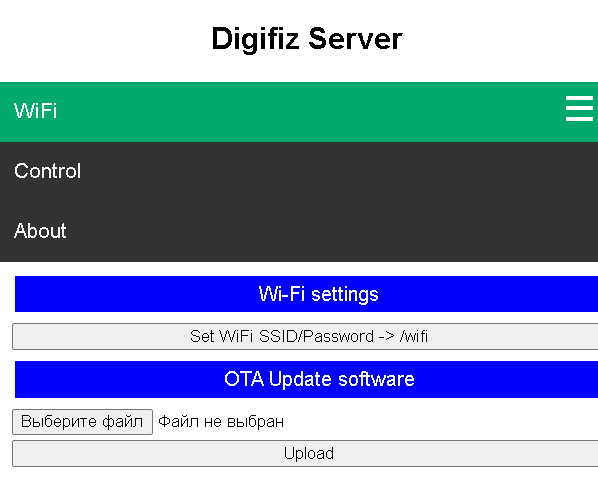
\includegraphics[width=\linewidth]{digifiz_manual/image020.png}
        \caption{Control tab overview.}
    \end{subfigure}\hfill
    \begin{subfigure}{0.48\textwidth}
        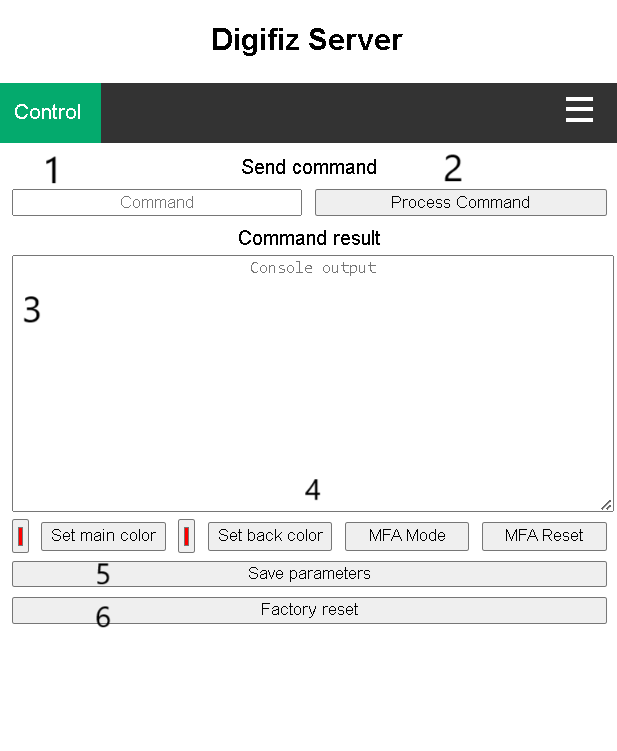
\includegraphics[width=\linewidth]{digifiz_manual/image021.png}
        \caption{Numbered controls and command entry fields.}
    \end{subfigure}
    \caption{\ReplicaNextShort{} Wi-Fi control interface.}
    \label{fig:next-control-tabs}
\end{figure}

\section{Command entry}
The \emph{Control} tab provides a command input line (1), a \emph{Process} button (2), a result window (3), quick controls (4), a \emph{Save} button (5), and a \emph{Reset} button (6). Enter commands as space-separated pairs \verb|<number> <value>| using integers only; punctuation and quotation marks are not required. \autoref{fig:next-command-example} illustrates the interface while toggling automatic brightness.

\begin{figure}[htbp]
    \centering
    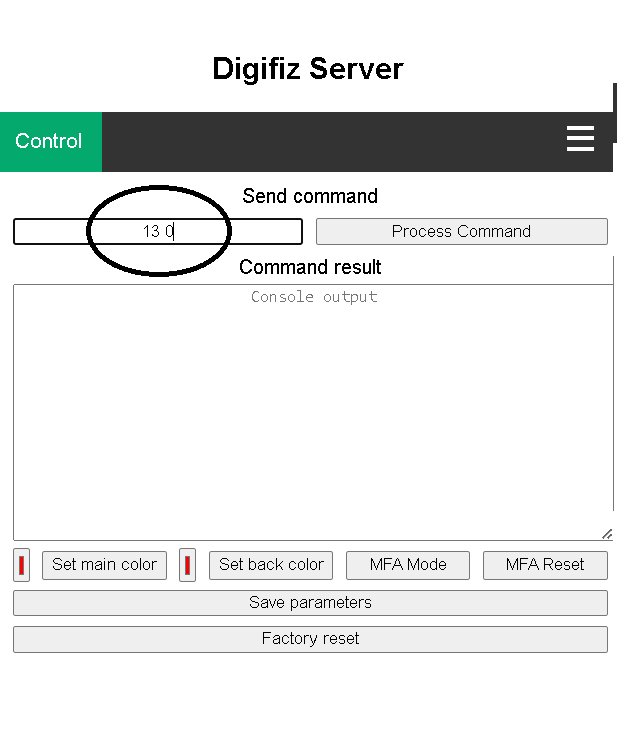
\includegraphics[width=0.55\textwidth]{digifiz_manual/image022.png}
    \caption{Example command sequence disabling automatic brightness.}
    \label{fig:next-command-example}
\end{figure}

\section{Command reference}
\begin{table}[htbp]
    \centering
    \caption{Primary \ReplicaNextShort{} configuration commands.}
    \label{tbl:next-commands}
    {\scriptsize
    \begin{tblr}{
        colspec = {Q[c,0.14\linewidth] >{\ttfamily}Q[l,0.36\linewidth] Q[l]},
        rowsep = 2pt,
    }
        \toprule
        \textbf{Command} & \textbf{Name} & \textbf{Description} \\
        \midrule
        22 (or 0) & PARAMETER\_RPMCOEFFICIENT & Engine RPM calibration factor (100--10000). \\
        1  & PARAMETER\_SPEEDCOEFFICIENT & Speed calibration factor (10--255). \\
        2  & PARAMETER\_COOLANTTHERMISTORB & Coolant thermistor beta coefficient (2000--5000). \\
        3  & PARAMETER\_OILTHERMISTORB & Oil thermistor beta coefficient (2000--5000). \\
        4  & PARAMETER\_AIRTHERMISTORB & Ambient thermistor beta coefficient (2000--5000). \\
        5  & PARAMETER\_TANKMINRESISTANCE & Minimum fuel sender resistance (0--1000~\ohm). \\
        6  & PARAMETER\_TANKMAXRESISTANCE & Maximum fuel sender resistance (100--1000~\ohm). \\
        7  & PARAMETER\_TAU\_COOLANT & Coolant temperature filter constant (1--50, higher is more responsive). \\
        8  & PARAMETER\_TAU\_OIL & Oil temperature filter constant (1--50). \\
        9  & PARAMETER\_TAU\_AIR & Ambient temperature filter constant (1--50). \\
        10 & PARAMETER\_TAU\_TANK & Fuel level filter constant (1--50). \\
        11 & PARAMETER\_MILEAGE & Total odometer value (0--999999). \\
        12 & PARAMETER\_DAILY\_MILEAGE & Trip odometer (0--9999). \\
        13 & PARAMETER\_AUTO\_BRIGHTNESS & Automatic brightness enable (1=on, 0=off). \\
        14 & PARAMETER\_BRIGHTNESS\_LEVEL & Manual brightness level (0--60\%; values above 60 reduce LED life). \\
        15 & PARAMETER\_TANK\_CAPACITY & Fuel tank capacity in litres (0--99; 55~L typical for Golf~2). \\
        16 & PARAMETER\_MFA\_STATE & Active MFA mode (normally controlled via hardware input). \\
        17 & PARAMETER\_BUZZER\_OFF & Disable buzzer (1 disables, 0 enables; \ReplicaNextShort{} lacks a buzzer). \\
        18 & PARAMETER\_MAX\_RPM & Tachometer scaling (typical 8000, range 4000--16000). \\
        19 & PARAMETER\_NORMAL\_RESISTANCE\_COOLANT & Coolant sensor resistance at \SI{25}{\celsius} (1000--10000~\ohm). \\
        20 & PARAMETER\_NORMAL\_RESISTANCE\_OIL & Oil sensor resistance at \SI{25}{\celsius} (1000--10000~\ohm). \\
        21 & PARAMETER\_NORMAL\_RESISTANCE\_AMB & Ambient sensor resistance at \SI{25}{\celsius} (1000--10000~\ohm). \\
        23 & PARAMETER\_DOT\_OFF & Clock colon behaviour (0=blink, 1=solid). \\
        24 & PARAMETER\_BACKLIGHT\_ON & Enable backlight on low beam (not used on \ReplicaNextShort{}). \\
        25 & PARAMETER\_M\_D\_FILTER & Median filter constant (legacy, normally unused). \\
        26 & PARAMETER\_COOLANT\_MAX\_R & Coolant sensor threshold for full-scale indication (\SI{100}{\celsius}--\SI{150}{\celsius}). \\
        27 & PARAMETER\_COOLANT\_MIN\_R & Coolant sensor threshold for ``1~bar'' indication (\SI{0}{\celsius}--\SI{80}{\celsius}). \\
        31 & PARAMETER\_MAINCOLOR\_R & Red component of the UI colour (0--255). \\
        32 & PARAMETER\_MAINCOLOR\_G & Green component of the UI colour (0--255). \\
        33 & PARAMETER\_MAINCOLOR\_B & Blue component of the UI colour (0--255). \\
        37 & PARAMETER\_RPM\_FILTER & RPM filter aggressiveness (10--200, higher reacts faster). \\
        128 & PARAMETER\_READ\_ADDITION & Add 128 to read the current value of any command. \\
        255 & PARAMETER\_SET\_HOUR & Set clock hours (24-hour format). \\
        254 & PARAMETER\_SET\_MINUTE & Set clock minutes. \\
        253 & PARAMETER\_RESET\_DAILY\_MILEAGE & Reset the trip odometer. \\
        252 & PARAMETER\_RESET\_DIGITAL & Factory reset of stored parameters. \\
        \bottomrule
    \end{tblr}}
\end{table}

\section{Default values}
\begin{table}[htbp]
    \centering
    \caption{\ReplicaNextShort{} default settings.}
    \label{tbl:next-defaults}
    {\scriptsize
    \begin{tblr}{
        colspec = {>{\ttfamily}Q[l,0.42\linewidth] Q[c,0.15\linewidth] Q[l]},
        rowsep = 2pt,
    }
        \toprule
        \textbf{Parameter} & \textbf{Default} & \textbf{Notes} \\
        \midrule
        PARAMETER\_RPMCOEFFICIENT & 3000 & Typical for Audi tachometer inputs. \\
        PARAMETER\_SPEEDCOEFFICIENT & 100 & Calibrated for 100~km/h. \\
        PARAMETER\_COOLANTTHERMISTORB & 4000 &  \\
        PARAMETER\_OILTHERMISTORB & 4000 &  \\
        PARAMETER\_AIRTHERMISTORB & 3812 & 3600 for Generation~2 panels. \\
        PARAMETER\_TANKMINRESISTANCE & 35 & \ohm. \\
        PARAMETER\_TANKMAXRESISTANCE & 265 & \ohm. \\
        PARAMETER\_TAU\_COOLANT & 2 & Filter constant. \\
        PARAMETER\_TAU\_OIL & 2 & Filter constant. \\
        PARAMETER\_TAU\_AIR & 2 & Filter constant. \\
        PARAMETER\_TAU\_TANK & 2 & Filter constant. \\
        PARAMETER\_MILEAGE & Vehicle-specific & Retains stored odometer. \\
        PARAMETER\_DAILY\_MILEAGE & 0 &  \\
        PARAMETER\_AUTO\_BRIGHTNESS & 1 & Enabled. \\
        PARAMETER\_BRIGHTNESS\_LEVEL & 25 & Generation~2 default; Generation~1/1.5 use 7 or 13. \\
        PARAMETER\_TANK\_CAPACITY & 63 & Litres. \\
        PARAMETER\_MFA\_STATE & 0 & Default MFA page. \\
        PARAMETER\_BUZZER\_OFF & 1 & Buzzer disabled. \\
        PARAMETER\_MAX\_RPM & 8000 & Tachometer scale. \\
        PARAMETER\_NORMAL\_RESISTANCE\_COOLANT & 1000 & \ohm{} at \SI{25}{\celsius}. \\
        PARAMETER\_NORMAL\_RESISTANCE\_OIL & 1000 & \ohm{} at \SI{25}{\celsius}. \\
        PARAMETER\_NORMAL\_RESISTANCE\_AMB & 2991 & 500~\ohm{} for Generation~2 sensors. \\
        PARAMETER\_DOT\_OFF & 0 & Blinking clock colon. \\
        PARAMETER\_BACKLIGHT\_ON & 1 & Backlight enabled with low beam. \\
        PARAMETER\_M\_D\_FILTER & 65535 & Legacy median filter constant. \\
        PARAMETER\_COOLANT\_MAX\_R & 120 & \si{\celsius}. \\
        PARAMETER\_COOLANT\_MIN\_R & 60 & \si{\celsius}. \\
        PARAMETER\_MAINCOLOR\_R & 180 & Yellow-green default. \\
        PARAMETER\_MAINCOLOR\_G & 240 & Yellow-green default. \\
        PARAMETER\_MAINCOLOR\_B & 6 & Yellow-green default. \\
        PARAMETER\_RPM\_FILTER & 70 & Filter response. \\
        PARAMETER\_UPTIME & 0 & Runtime counter. \\
        \bottomrule
    \end{tblr}}
\end{table}

\section{Reading parameters and examples}
To read a parameter, add 128 to the command number (for example, \verb|129 0| reports the speed coefficient). Typical commands include disabling automatic brightness (\verb|13 0|), enabling it again (\verb|13 1|), adjusting the speed coefficient (\verb|1 110| increases the displayed speed by 10\%), and setting the odometer (\verb|11 123456|). Clock values are set with \verb|255 <hours>| followed by \verb|254 <minutes>|. Commands 31--33 set the RGB components of the user interface colour.

\section{Service commands}
Recent firmware revisions accept human-readable parameter names, for example \verb|PARAMETER_RPMCOEFFICIENT 3000|. The diagnostic command \verb|adc 0| prints raw ADC readings for sensor troubleshooting. Firmware updates add visual colour controls, so update regularly through the \emph{WiFi} tab to access the latest features.
